\documentclass[a4paper]{article} %%% use \documentstyle for old LaTeX compilers

\usepackage[portuguese]{babel} %%% 'french', 'german', 'spanish', 'danish', etc.
\usepackage{makeidx}
\usepackage{multirow}
\usepackage{multicol}
\usepackage[dvipsnames,svgnames,table]{xcolor}
\usepackage[dvips]{graphicx} 
\usepackage{epstopdf}
\usepackage{ulem}
\usepackage{hyperref}
\usepackage{amsmath}
\usepackage{amssymb}
\usepackage{txfonts}
\usepackage{mathdots}
\usepackage[classicReIm]{kpfonts}

% You can include more LaTeX packages here 

\author{Bruno da silva}

\usepackage[a4paper,top=2.5cm,bottom=2.5cm,left=3cm,right=3cm,marginparwidth=1.75cm]{geometry}

\begin{document}

%\selectlanguage{english} %%% remove comment delimiter ('%') and select language if required


\fontfamily{phv}\selectfont

\begin{center}
	{\Large Universidade Federal Fluminense -UFF}
\end{center}
\begin{center}
	\
\end{center}
\begin{center}
	\
\end{center}
\begin{center}
	\
\end{center}
\begin{center}
	\
\end{center}
\begin{center}
	\
\end{center}
\begin{center}
	\
\end{center}
\begin{center}
	\
\end{center}
\begin{center}
	\
\end{center}
\begin{center}
	\
\end{center}
\begin{center}
	{\Large Pendulo com arrasto
	}
\end{center}
\begin{center}
	\
\end{center}
\begin{center}
	\
\end{center}
\begin{center}
	\
\end{center}

\begin{center}
\end{center}

\begin{center}
	\
\end{center}
\begin{center}
	\
\end{center}
\begin{center}
	\
\end{center}


\begin{center}
	Autor Bruno da Silva Machado
\end{center}
\begin{center}
	\
\end{center}
\begin{center}
	\
\end{center}
\begin{center}
	\
\end{center}
\begin{center}
	\
\end{center}
\begin{center}
	\
\end{center}
\begin{center}
	\
\end{center}

\begin{center}
	\
\end{center}
\begin{center}
	\
\end{center}
\begin{center}
	\
\end{center}
\begin{center}
	Volta Redonda 15 de maio 2017\eject 
	
\end{center}

\setcounter{secnumdepth}{0}
\section{Introdu\c{c}\~{a}o}
\noindent

Neste trabalho, estudaremos o pendulo com arrasto admitindo uma for\c{c}a de atrito viscoso, que depende somente da velocidade angular. 
\noindent \eject 

\section{Pendulo com arrasto}
\noindent 

Em mec\^anica, um p\^endulo f\'isico pode ser chamado de p\^endulo real, pois n\~ao tem uma distribui\c{c}\~ao uniforme de massa. Ele consiste em um objeto que oscila em torno de um eixo de rota\c{c}\~ao perpendicular ao plano em que se movimenta. No caso do p\^endulo com arrasto temos uma for\c{c}a adicional oposta proporcional a velocidade. O p\^endulo \'e muito utilizado em estudos da for\c{c}a peso e do movimento oscilat\'orio.

De acordo com Halliday e Resnick, 2009, quando o movimento de um oscilador \'e reduzido por uma for\c{c}a externa dizemos que o seu movimento \'e amortecido. A constante de amortecimento depende das caracter\'isticas, tanto do p\^endulo quanto do meio em que se encontra oscilando.

\begin{center}
	\includegraphics[width=1.88in,height=2.55in,keepaspectratio = false]{pendulo.png}
	
	\scriptsize Figura 1. p\^endulo f\'isico fora da poci\c{c}\~ao de equil\'ibrio. Observe a for\c{c}a de arrasto e oposta ao movimento
	
\end{center}

O Pendulo, apresentado na figura 1, est\'a sujeito as seguintes hip\'oteses:
\begin{enumerate}
\item A massa pendular est\'a concentrada apenas no elemento oscilante;
\item A haste n\~ao possui massa, \'e inextens\'ivel e inflex\'ivel;
\item O movimento pendular aconteceem torno de um eixo de rota\c{c}\~ao perpendicular ao plano em que se movimenta;
\item O movimento pendular n\~ao \'e conservativo (h\'a for\c{c}a de atrito).
\end{enumerate}

\section{Solu\c{c}\~ao do Pendulo}

Quando um p\^endulo \'e deslocado do seu ponto de equil\'ibrio, for\c{c}a externas passam a agir sobre o mesmo, entre elas est\'a um torque restaurador devido ao peso do corpo buscando restaurar o p\^endulo para suapoci\c{c}\~ao de equil\'ibrio, com isso temos que:
\[ \sum{T} = I\dot{\theta} \]
onde:
\[ I = \int{L^2dm} = L^2m \]
\[ \sum{T} = -mgL\sin(\theta) - k\dot{\theta} \]
logo,
\[-mgL\sin(\theta) - k\dot{\theta} = L^2m\dot{\theta}\]

dividindo por $mL^2$,obtemos:
\[-\frac{g}{L}\sin(\theta) - \frac{k}{mL^2}\dot{\theta} = \dot{\theta}\]
fazendo $\omega^2 = \frac{g}{L}$ e $\gamma = \frac{k}{mL^2}$ temos
\[-\omega^2\sin(\theta) - \gamma\dot{\theta} = \dot{\theta}\](1)

Note que esta e uma EDO \textbf{n\~ao linear} do p\^endulo, mas se considerarmos pequenos \^angulos para seno podemos reescreve-la como
\[-\omega^2\theta - \gamma\dot{\theta} = \dot{\theta}\](2)

sendo esta uma solu\c{c}\~ao linear, ou seja possui resolu\c{c}\~ao.

 utilizando m\'etodo de Verlet obtemos a seguinte solu\c{c}\~ao numerica

\[ x_{t+1} = x_t + v_tt + 1/2a_t(\Delta{t})^2 \]
\[a_{tmp} = a(x_{t+1}, v_t)\]
\[v_{tmp} = v_t + 1/2(a_t + a_{tmp})\Delta{t}\]
\[a_{tmp} = a(x_{t+1}, v_{tmp})\]
\[v_{t+1} = v_t + 1/2(a_t + a_{tmp})\Delta{t}\]
\[a_{t+1} = a(x_{t+1}, v_{t+1})\]

\section{Resultado}

Nas figuras a seguir vamos visualizar as solu\c{c}\~oes obtidas na se\c{c}\~ao anterior, nelas est\~ao representadas a posi\c{c}\~ao, velocidade e espa\c{c}o de fase do p\^endulo para o caso em que frequ\^encia angular $\omega^2$ \'e igual a 3,5 e 10, com o constante de arrasto $\gamma$ igual a 0.1, 0.5 e 1.0 e a  posi\c{c}\~ao inicial $x_0 = 1$m com velocidade $v_0 = 0$. Nestes gr\'aficos, podemos notar que a posi\c{c}~ao e a velocidade s\~ao cont\'inuas embora a modula\c{c}~ao da amplitude n\~ao seja,Tamb\'em notamos que suas amplitudes decrescem de forma inst\'avel com o tempo.

\begin{center}
	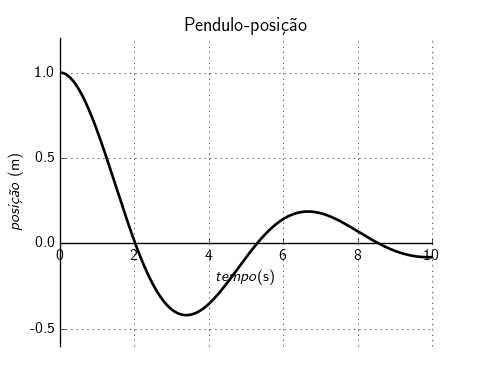
\includegraphics[width=4.80in,height=3.84in,keepaspectratio = false]{pendulo1_image1.png}
	
	\scriptsize Figura 2. 
\end{center}
\begin{center}	
	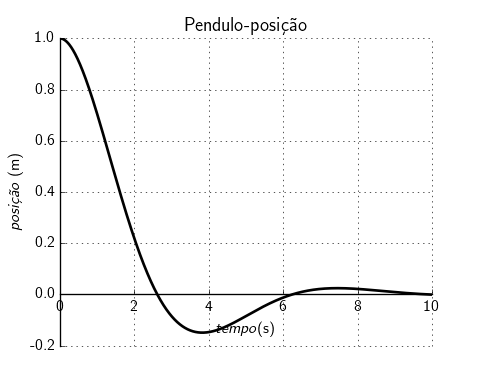
\includegraphics[width=4.80in,height=3.84in,keepaspectratio = false]{pendulo2_image1.png}
	
	\scriptsize Figura 3. 
\end{center}
\begin{center}	
	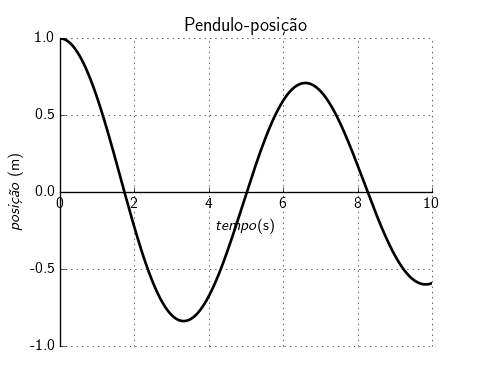
\includegraphics[width=4.80in,height=3.84in,keepaspectratio = false]{pendulo3_image1.png}
	
	\scriptsize Figura 4. 
	
\end{center}

Nas figuras 2,3 e 4 temos gr\'afico da Posi\c{c}\~ao x Tempo do pendulo - A linha cont\'inua representa a oscila\c{c}\~ao do corpo, que se mant\'em at\'e que o torque restaurador feito pele pendulo em um ponto de retorno seja menor que a for\c{c}a de arrasto m\'axima.


\begin{center}
	
	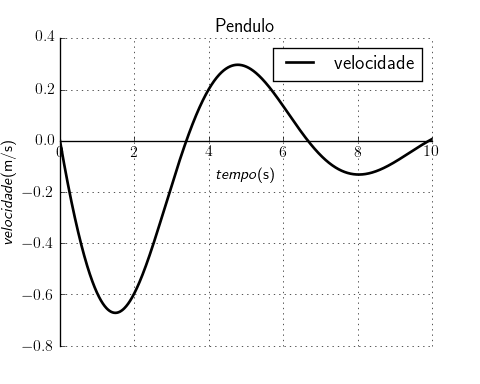
\includegraphics[width=4.80in,height=3.84in,keepaspectratio = false]{pendulo1_image2.png}
	
	\scriptsize  Figura 5. 
	
	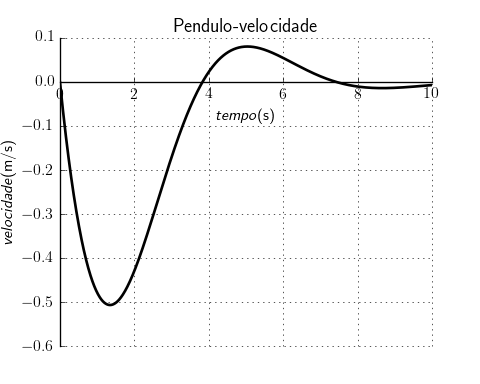
\includegraphics[width=4.80in,height=3.84in,keepaspectratio = false]{pendulo2_image2.png}
	
	\scriptsize  Figura 6. 
	
	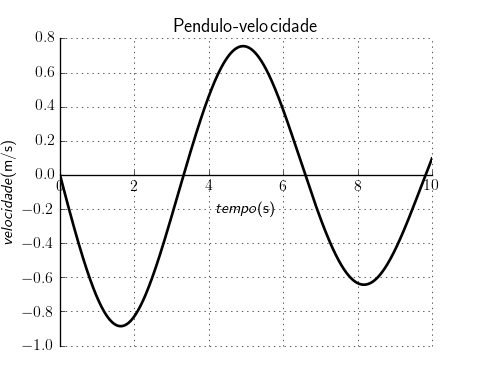
\includegraphics[width=4.80in,height=3.84in,keepaspectratio = false]{pendulo3_image2.png}
	
	\scriptsize  Figura 7. 
	
\end{center}

Nas figuras 5,6,e7 vemos os gr\'aficos da Velocidade x Tempo do pendulo - Podemos notar que a velocidade m\'axima em cada semi-ciclo decresce com o tempo, tem a forma senoidal e a mudan\c{c}a de amplitude ocorre nos pontos em que a velocidade \'e nula.
 
\begin{center}
	
	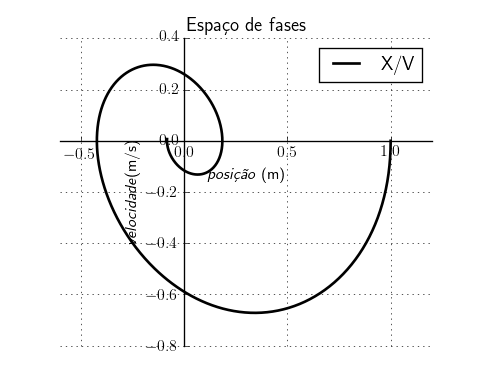
\includegraphics[width=4.80in,height=3.84in,keepaspectratio = false]{pendulo1_image3.png}
	
	\scriptsize  Figura 8. 
	
	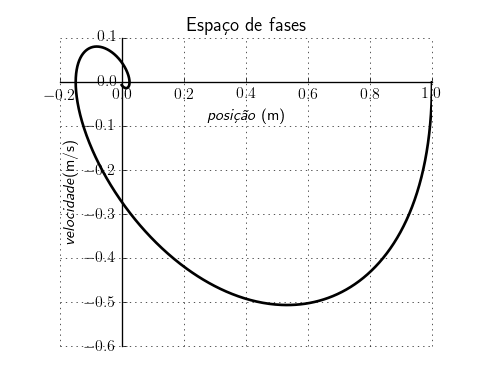
\includegraphics[width=4.80in,height=3.84in,keepaspectratio = false]{pendulo2_image3.png}
	
	\scriptsize  Figura 9. 
	
	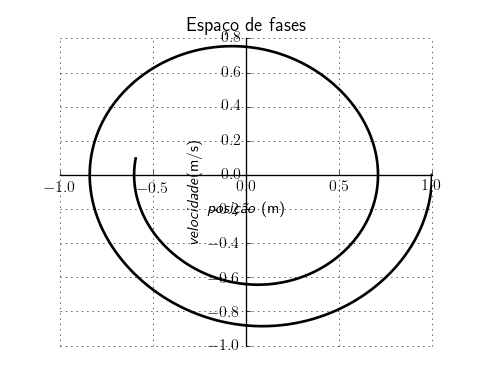
\includegraphics[width=4.80in,height=3.84in,keepaspectratio = false]{pendulo3_image3.png}
	
	\scriptsize  Figura 10. 
		
\end{center}

Nas figuras 8,9 e 10 espa\c{c}o de fase do pendulo com arrasto a patir dele podemos supor que a energia do oscilador n\~ao se conserva uma vez que a curva n\~ao fechada e tem um formato de espiral.

Como j\'a sabemos a energia se dissipa com o tempo atraves do espa\c{c}o de configura\c{c}\~ao vimos que ela decai de maneira suave e na forma de espiral. configura\c{c}\~oes desse tipo s\~ao caracter\'isticas quando a energia possui depend\^encias trigonom\'etricas.
podemos assim definir a energia como soma da cin\'etica com a potencial
Temos:
\[T = \frac{1}{2}m\dot{\theta}\]
e
\[U = mgl\cos(\theta)\]
\[U = \frac{m\omega^2}{g}cos(\theta)\]
pressupondo a naureza do problema sabemos que a energia decai exponencialmente com o tempo, para confirmar nossa suspeitas fa\c{c}amos um gr\'afico. 

\begin{center}
	
	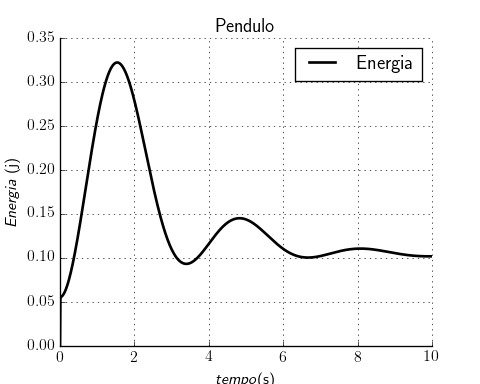
\includegraphics[width=4.80in,height=3.84in,keepaspectratio = false]{pendulo1_image4.png}
	
	\scriptsize  Figura 11. gr\'afico da energia contra o tempo 
\end{center}

\section{Conclu\c{c}\~ao}

Nesse trabalho estudamos o comportamento do pendulo real e apresentamos a solu\c{c}\~ao para \^angulos em que $\sin(\theta) > \theta$ e pequenos com uma for\c{c}a dissipativa depende de um coeficiente de arrasto e do m\'odulo da velocidade, tambem verificamos que a amplitude decai exponencialmente assim como a energia. E atrav\'es do m\'etodos de Verlet podemos fazer uma analise numerica do problema e encontrando facilmente a sua solu\c{c}\~ao 

\section{Referencia}

\noindent 
\indent 1. a) D. HALLIDAY e R. RESNICK, Fundamentos de F\'isica, vol. 2, Livros T\'ecnicos e Cient\'ificos, Rio de Janeiro, 1991. b) P. TIPLER, F\'isica, vol. 2, 3a ed., Guanabara Koogan, Rio de Janeiro, 1991.

\indent 2. J. B. MARION, Classical Dynamics, 2a ed., Academic Press, New York, 1965.

\indent 3. J.-J. E. Slotine, W. Li, "Applied nonlinear control", Prentice-Hall, Englewood Cliffs, New Jersey, 1991.

\indent 4. M. A. Savi, "Din\^amica n\~ao-linear e caos", E-papers, Rio de Janeiro, 2006.


\end{document}

